%%%%%%%%%%%%%%%%%%%%%---Chapter6 Formatting---%%%%%%%%%%%%%%%%%%%%%%%%%%%%%%%%%%
\documentclass[Thesis.tex]{subfiles}
\begin{document}
\setcounter{chapter}{5} %%Chapter Numbering


%%%%%%%%%%%%%%%%%%%%%%%%%%%%%%%%%%%%%%%%%%%%%%%%%%%%%%%%%%%%%%%%%%%%%%%%%%%%

\chapter{Results: Machine-Learning Syndrome Decoding}\label{chap6:decoding}

This chapter compares learned syndrome decoders with model-based baselines.
Minimum-weight perfect matching (MWPM) minimises the fault count for this
equal-rate noise model. Exact maximum a posteriori (MAP) decoding minimises
the expected logical error for the known model.
The comparison asks how much the choice of objective affects performance.

\section{Scope of this chapter}\label{sec:ch6_scope}

The experiment is a simulated bit-flip memory for the distance-$d$ repetition
code under phenomenological noise. Its fault mechanisms give an explicit
space-time detector graph, and the small codes allow exact calculation of logical
class probabilities. The logical error rates and finite-distance crossover
diagnostics in this chapter refer to this memory experiment and its noise model.

\section{Methodology}\label{sec:ch6_method}

\subsection{Noise model and sampling}

The code uses $d$ data qubits and $d-1$ adjacent parity checks. In each of $T=d$
rounds, each data qubit incurs a bit flip independently with probability $p$ and each check
measurement is independently misreported with the same probability. The data
errors accumulate by exclusive-or. The experiment ends with a perfect data
readout, giving one final check value for each parity and no additional data or
measurement faults. A detector records the difference between consecutive
observed check values, starting from the known zero syndrome. There are
$(T+1)(d-1)$ detectors per shot and the logical observable is the accumulated
error on the first data bit.

The sweep uses $d\in\{3,5,7,9\}$. The physical error rates are $0.01$, $0.02$,
$0.03$, $0.04$, $0.05$, $0.06$, $0.08$, $0.10$, $0.12$, and $0.15$.
For each of the $40$ configurations, the simulator generates $400{,}000$ shots,
split into disjoint $200{,}000$-shot training and test blocks, for $16$ million
generated shots. All model-based decoders and classical learned decoders run
on the entire test block. The MLP reserves $10\%$ of the training block for
early stopping. The simulator-based VQC uses a $15{,}000$-shot labelled
training block and reserves $1{,}500$ of those shots for validation. It uses the
first $50{,}000$ test shots. The result table also records every decoder's
error on that common $50{,}000$-shot prefix.

\subsection{Matching on the detector graph}

A single interior data fault produces a horizontal edge between two adjacent
detectors in the same noisy round. A data fault on the first or last bit gives
a spatial-boundary edge, and only a first-bit fault flips the logical
observable. A check measurement fault connects the corresponding detector
in that round to its successor. Consequently, the final detector row has only
vertical links to the preceding row. Its spatial links are absent because the
simulator injects no data faults at the perfect readout.

MWPM uses the sparse blossom implementation in PyMatching
2.4.0~\cite{higgott2022pymatching,higgott2025sparseblossom}.
Each allowed elementary fault has the same weight
$\log((1-p)/p)>0$, so unit weights give the same minimisers.
The decoder returns the logical parity of the selected correction. Greedy
matching first accounts for the forced links at final-row defects. On the
remaining graph it repeatedly chooses the shortest available defect--defect
or defect--boundary path, with a fixed ordering for equal lengths. When
several MWPM corrections have equal cost, they can differ in logical class.

At $d=3$, the $9$ data-fault locations and $6$ measurement-fault locations make
exhaustive validation possible. Enumerating all $2^{15}=32{,}768$ fault
histories yields the minimum weight for each logical class for every one of
the $256$ syndromes. PyMatching attained the physical minimum and returned
an eligible logical class for every syndrome. The two logical classes have
equal minimum fault counts for $104$ of the $256$ syndromes. Single-fault
checks also verified the detector patterns and logical flags at all four
distances.

\subsection{Exact logical-class posterior}

The exact MAP decoder uses the simulator's value of $p$. It reconstructs the
observed check string $m_t$ after round $t$ by accumulating detector differences.
Let $e_t$ be the cumulative data-error string and $s(e_t)$ its adjacent parities.
Write $w_t(e)$ for the joint probability of state $e_t=e$ and the noisy check
history through round $t$. With $w_0(e)=\mathbf{1}_{e=0}$ and
$h_t(e)=|m_t\oplus s(e)|$, the update is given by Eq.~\eqref{eq:ch6_posterior_update},
\begin{equation}
  w_t(e)=p^{h_t(e)}(1-p)^{d-1-h_t(e)}
  \sum_{e'} w_{t-1}(e')\,p^{|e\oplus e'|}(1-p)^{d-|e\oplus e'|},
  \label{eq:ch6_posterior_update}
\end{equation}
where $|\cdot|$ denotes Hamming weight. The implementation factors the transition
into $d$ single-bit updates over the $2^d$ states. The perfect final check restricts the
last state to $s(e_T)=m_{T+1}$. This leaves two complementary data-error
strings, one for each value of the first bit. The decoder predicts the more
probable logical class after normalising the two remaining weights. The control
uses no fitted parameters, and the state count grows exponentially with
distance. The same distance-3 fault enumeration provides an independent
check of the posterior. The maximum absolute discrepancy in the conditional
probabilities across all syndromes and sampled rates is below $1.3\times10^{-15}$.

Thus, MWPM minimises the weight of an individual explanation of the syndrome.
Exact MAP sums the probability of all explanations within each logical class.
A class with more compatible fault histories can have higher posterior
probability even when its lightest individual history requires more faults.

\subsection{Model arms and comparisons}

Table~\ref{tab:ch6_decoders} summarises the seven decoders. Code distance and
physical noise rate are fixed within each train/test comparison.

\begin{table}[htbp]
\centering
\caption[Decoders benchmarked]{Trainable predictor parameters at $d=3$. The counts exclude PCA preprocessing. For the flat-syndrome logistic regression and MLP, the counts rise to $81$ and $18{,}689$ at $d=9$.}
\label{tab:ch6_decoders}
\small
\begin{tabular}{@{}>{\raggedright\arraybackslash}p{2.15cm} >{\raggedright\arraybackslash}p{2.15cm} >{\raggedright\arraybackslash}p{6.1cm} r@{}}
\toprule
\textbf{Decoder} & \textbf{Family} & \textbf{Description} & \textbf{Params} \\
\midrule
MWPM & combinatorial & Exact matching on the detector graph in PyMatching & 0 \\
Greedy & combinatorial & Shortest available connection on the same graph & 0 \\
Exact MAP & model-based & Forward recursion and logical-class marginalisation & 0 \\
Logistic reg. & learned & Logistic regression on the flattened syndrome & 9 \\
MLP & learned & Two hidden layers $(128,64)$, ReLU, Adam, early stopping & 9473 \\
Logistic reg., PCA & learned & Logistic regression on six PCA components & 7 \\
VQC, PCA & hybrid & Six-qubit, three-layer reuploading circuit with a sigmoid readout on $\langle Z_0\rangle$ & 38 \\
\bottomrule
\end{tabular}
\end{table}

The logical error rate (LER) is the fraction of test shots with an incorrect
logical bit. Wilson intervals describe the sampling uncertainty of each rate.
Between-decoder comparisons use paired correctness on the same shots
and exact McNemar tests on the discordant outcomes. Each comparison uses
the largest shared test prefix, with Holm's correction across the $280$
tests of the six alternatives versus MWPM and the MLP versus exact MAP.
These intervals and tests quantify held-out shot variation for the fitted
decoders. Training-set and optimiser variability are outside this calculation.
Very small McNemar $p$-values can round to zero in the result CSV.

\section{Logical error rates and finite-distance crossings}\label{sec:ch6_threshold}

\begin{figure}[!htb]
\centering
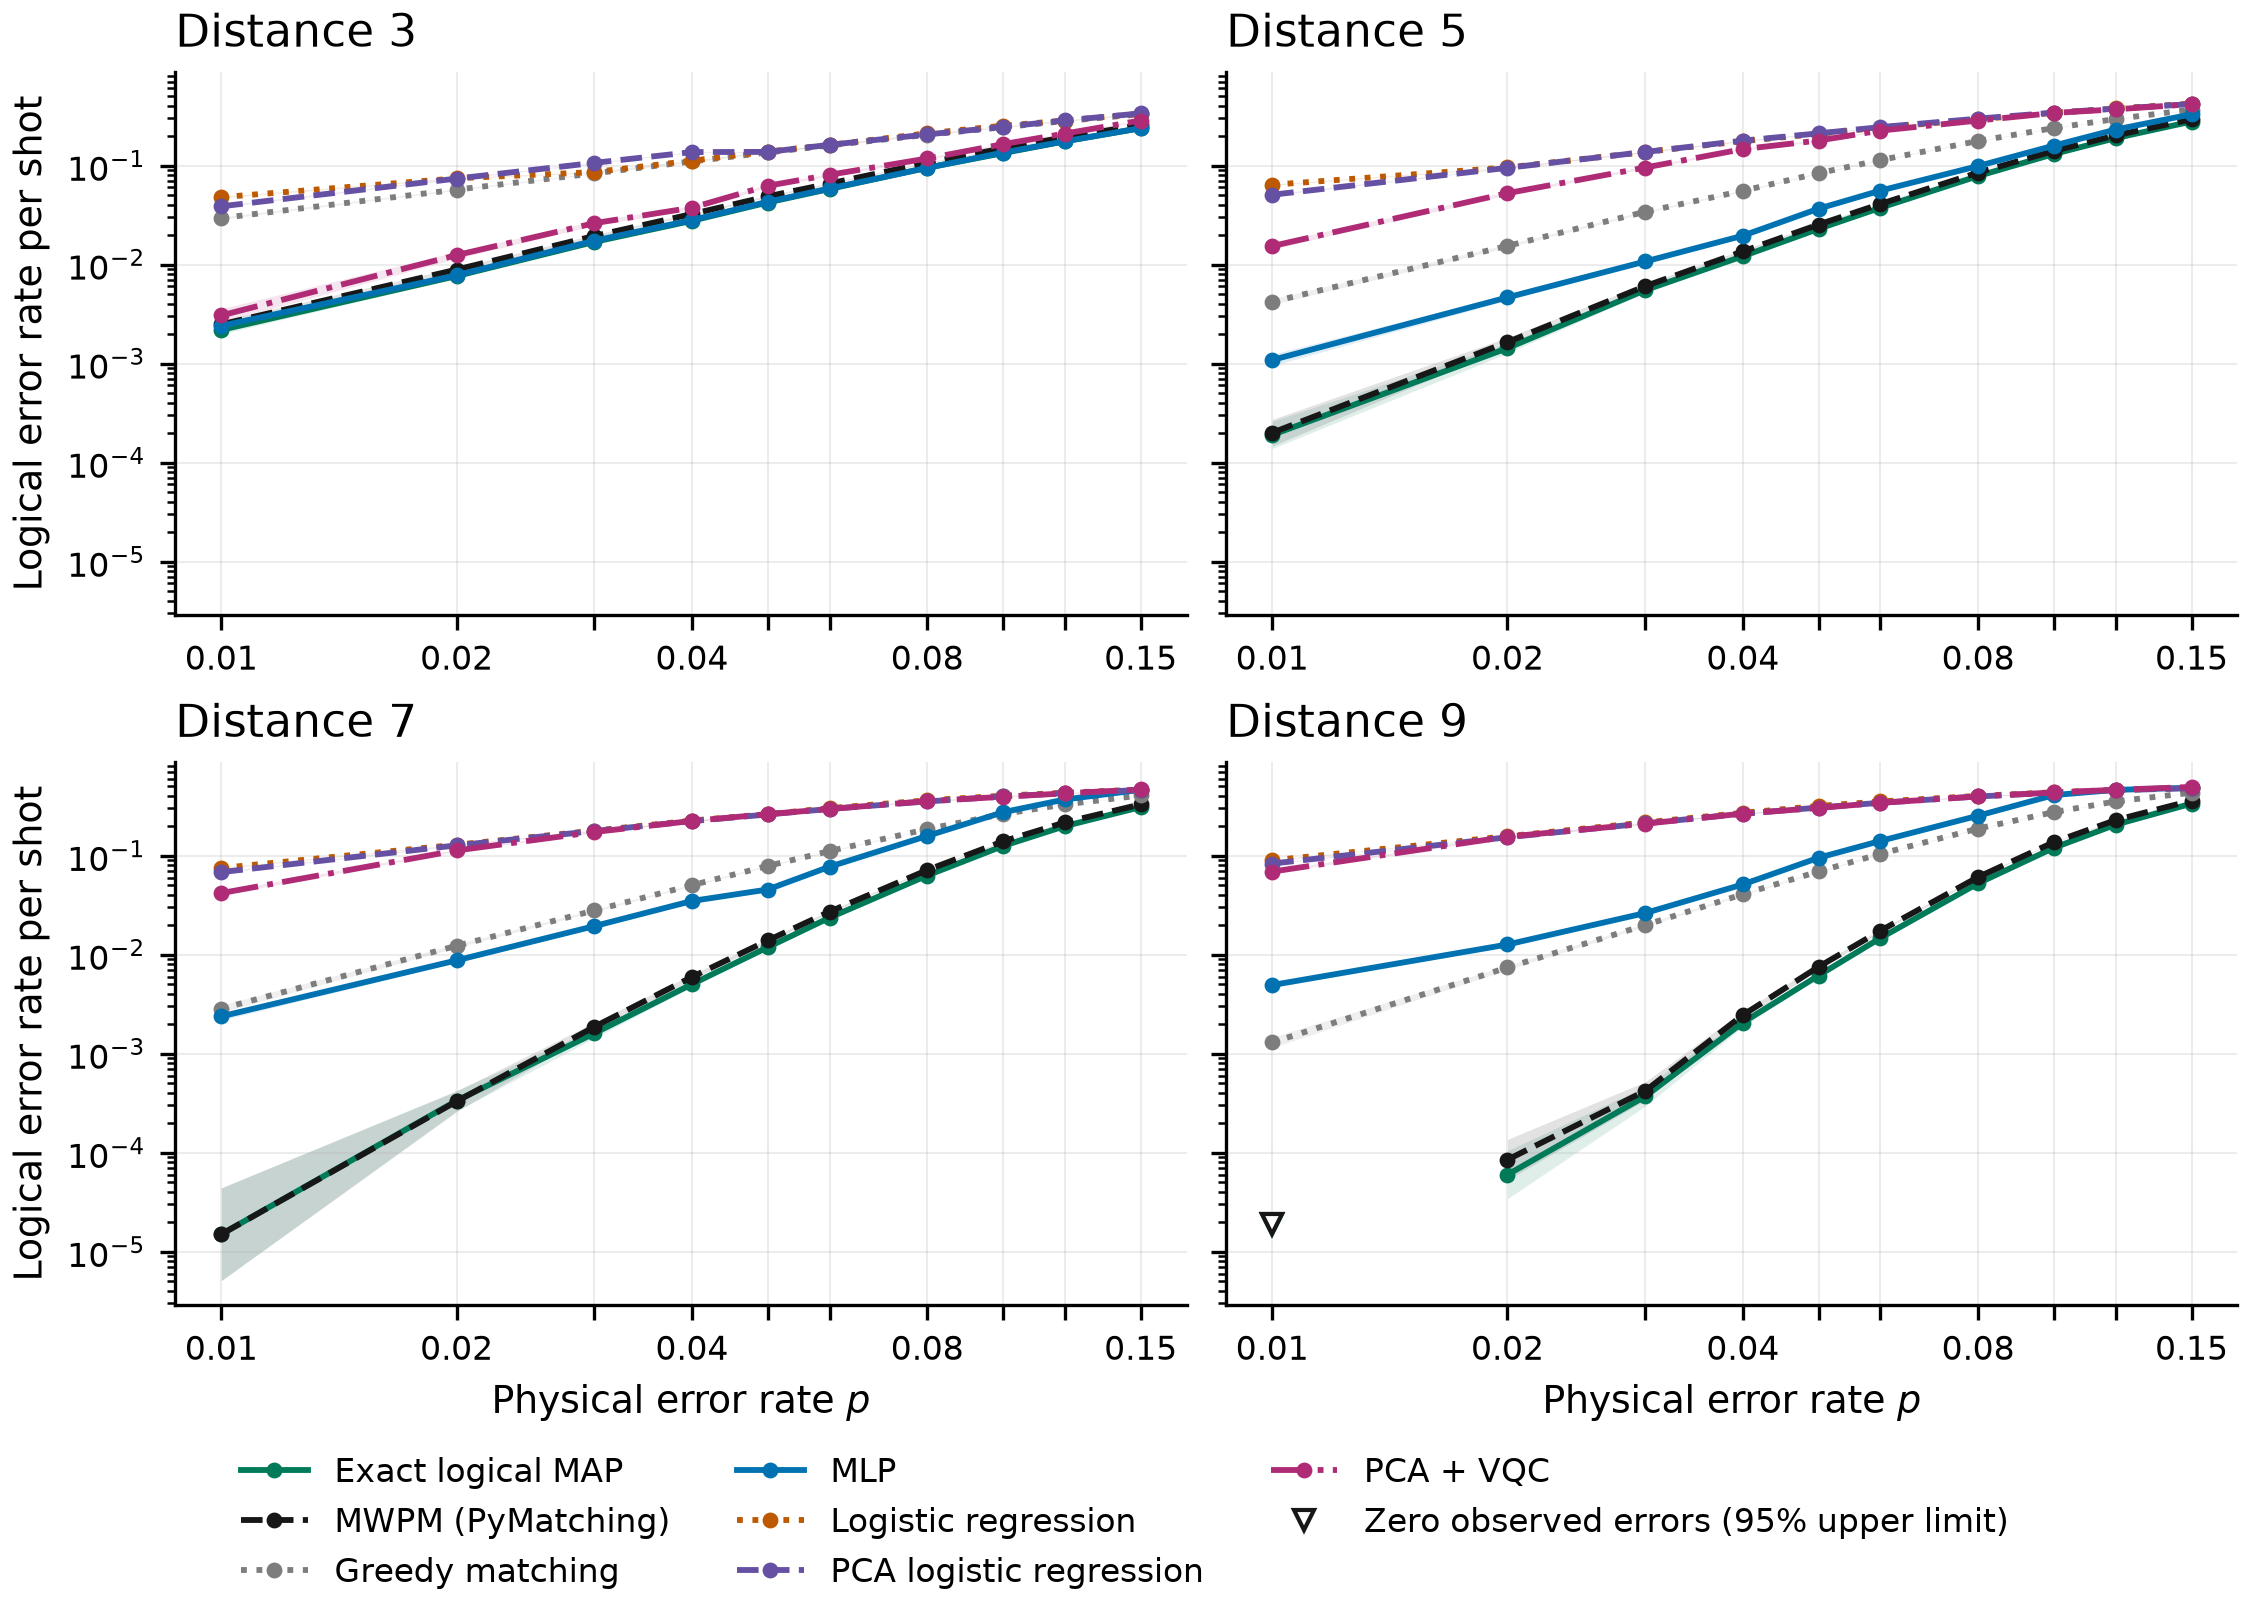
\includegraphics[width=\textwidth]{figures/ch6/qec_threshold_fig.png}
\caption[Logical error rate against physical error rate]{Logical error rate per shot at each physical error rate and code distance. Each arm uses its available test shots. Bands give Wilson $95\%$ intervals, and open triangles mark the Wilson upper bounds for zero observed errors.}
\label{fig:ch6_threshold}
\end{figure}

Figure~\ref{fig:ch6_threshold} shows the logical error rate of each decoder against the
physical error rate at every code distance.
At $p=0.02$, the simulated logical error falls at each distance step for
exact MAP, MWPM and greedy matching. From $d=3$ to $d=9$, exact MAP falls from
$0.007645$ to $0.000060$, and MWPM from $0.008890$ to $0.000085$.
The MLP improves from $0.007795$ at $d=3$ to $0.004655$ at $d=5$, then
rises to $0.008760$ at $d=7$ and $0.012670$ at $d=9$.
Figure~\ref{fig:ch6_comparison} shows the distance trends at this noise rate.

Table~\ref{tab:ch6_threshold} reports two descriptive diagnostics for the
change in direction with distance. For each adjacent pair, the procedure
keeps positive, unequal logical error rates and interpolates the first
reversal of their order in log-log coordinates. It averages the resulting
crossings over the pairs for which it finds a reversal. The finite-size
scaling (FSS) fit uses $p_L=F((p-p_{\mathrm{th}})d^{1/\nu})$ and fits a
quadratic $F$ by unweighted least squares on the measured rates at or above
$0.01$. It uses a bounded nonlinear fit with multiple initialisations.
The table omits a scaling fit when the decoder has neither a detected
crossing nor a lower observed error at $d=9$ than at $d=3$ for any sampled rate.
Both diagnostics depend on the sampled noise grid and the four tested
distances. The FSS fit also depends on the error-rate cutoff, and the table
gives point estimates without uncertainty on $p_{\mathrm{th}}$ or $\nu$.

\begin{table}[htbp]
\centering
\caption[Finite-distance crossover diagnostics]{Finite-distance crossover
diagnostics. Crossings is the mean over available adjacent-distance pairs.
A dash marks an estimate omitted by the stated criteria. The MLP scaling
fit is included as a sensitivity diagnostic for the single observed crossing.}
\label{tab:ch6_threshold}
\small
\begin{tabular}{lrrr}
\toprule
\textbf{Decoder} & \textbf{Crossings} & \textbf{FSS fit} & \textbf{$\nu$} \\
\midrule
MWPM & 0.1057 & 0.1031 & 1.87 \\
Greedy & 0.0824 & 0.0803 & 2.07 \\
Exact MAP & 0.1078 & 0.1047 & 1.91 \\
MLP & 0.0701 & 0.0231 & 1.19 \\
Logistic reg. & --- & --- & --- \\
Logistic reg., PCA & --- & --- & --- \\
VQC, PCA & --- & --- & --- \\
\bottomrule
\end{tabular}
\end{table}

The observed logical error rates of exact MAP and MWPM fall at every
distance step up to $p=0.10$ and rise at every step from $p=0.12$.
Their pairwise crossing estimates lie within $0.1013$--$0.1110$. Greedy
matching has a wider spread, $0.0654$--$0.1052$, about a mean of $0.0824$.
The MLP has one crossing, between $d=3$ and $d=5$, and a substantially lower
FSS estimate. It shows no monotonic improvement across all four distances at
any sampled rate. An asymptotic threshold or a critical exponent would
require a broader distance sweep and an uncertainty analysis.

\section{Comparing matching, learned decoders and MAP}
\label{sec:ch6_mlwin}

Across the $40$ configurations on the shared $50{,}000$-shot prefix, exact MAP
has the lowest observed error in $35$ outright and ties MWPM in one. MWPM and
the MLP each rank first outright in two configurations. The paired tests
against each reference use the largest shared prefix for that pair.
On those $200{,}000$-shot comparisons, exact MAP has lower error than MWPM
in $37$ configurations, with $34$ differences resolved after Holm
adjustment. The two methods tie in two configurations. MWPM has lower
observed error in one configuration, with no resolved difference there.
The MLP has lower error than MWPM at all ten rates at $d=3$,
with nine resolved differences, and has higher error at all $30$ larger-code
configurations. No comparison resolves an MLP improvement over exact MAP.
Table~\ref{tab:ch6_d3} lists the distance-3 rates of the three methods.

\begin{table}[htbp]
\centering
\caption[Distance-3 comparison on common test shots]{Distance-3 comparison of corrected matching, the MLP and exact logical-class decoding. The three methods were scored on the same $200{,}000$ test shots for each $p$. An asterisk denotes a Holm-adjusted paired test result below $0.05$.}
\label{tab:ch6_d3}
\small
\begin{tabular}{@{}lrrrr@{}}
\toprule
\textbf{$p$} & \textbf{MWPM LER} & \textbf{MLP LER} & \textbf{Exact MAP LER}
& \shortstack{\textbf{MLP minus}\\\textbf{MWPM}} \\
\midrule
0.01 & 0.002485 & 0.002405 & 0.002185 & $-0.000080$ \\
0.02 & 0.008890 & 0.007795 & 0.007645 & $-0.001095^{*}$ \\
0.03 & 0.019425 & 0.017420 & 0.016905 & $-0.002005^{*}$ \\
0.04 & 0.032360 & 0.028120 & 0.027635 & $-0.004240^{*}$ \\
0.05 & 0.048790 & 0.043000 & 0.042290 & $-0.005790^{*}$ \\
0.06 & 0.065785 & 0.058655 & 0.057930 & $-0.007130^{*}$ \\
0.08 & 0.106330 & 0.094740 & 0.094905 & $-0.011590^{*}$ \\
0.10 & 0.149035 & 0.135135 & 0.133345 & $-0.013900^{*}$ \\
0.12 & 0.192845 & 0.175760 & 0.175525 & $-0.017085^{*}$ \\
0.15 & 0.256485 & 0.238735 & 0.237845 & $-0.017750^{*}$ \\
\bottomrule
\end{tabular}
\end{table}

At $d=3$ and $p=0.15$, PyMatching, the MLP and exact MAP have test logical error
rates of $25.6485\%$, $23.8735\%$ and $23.7845\%$, respectively. At $p=0.08$
the MLP is $0.0165$ percentage points below exact MAP on the test sample.
The paired comparison has an unadjusted $p$-value of $0.56$ and the sampled reversal is
consistent with finite-shot variation.

The model gives an analytical check on the distance-3 result.
At $p=0.15$, the expected logical error of PyMatching is $25.6373\%$. Across
all legal choices among tied minimum-weight corrections, expected error
spans $23.7777\%$ to $27.1637\%$. At each of the ten sampled noise rates, the lower end of this tie range equals the exact MAP risk. Hence tie resolution accounts for
the gap between fixed PyMatching and exact MAP at this distance. The MLP's
performance falls between them at $p=0.15$. Figure~\ref{fig:ch6_comparison}
shows the analytical range across the sweep.

\begin{figure}[!htb]
\centering
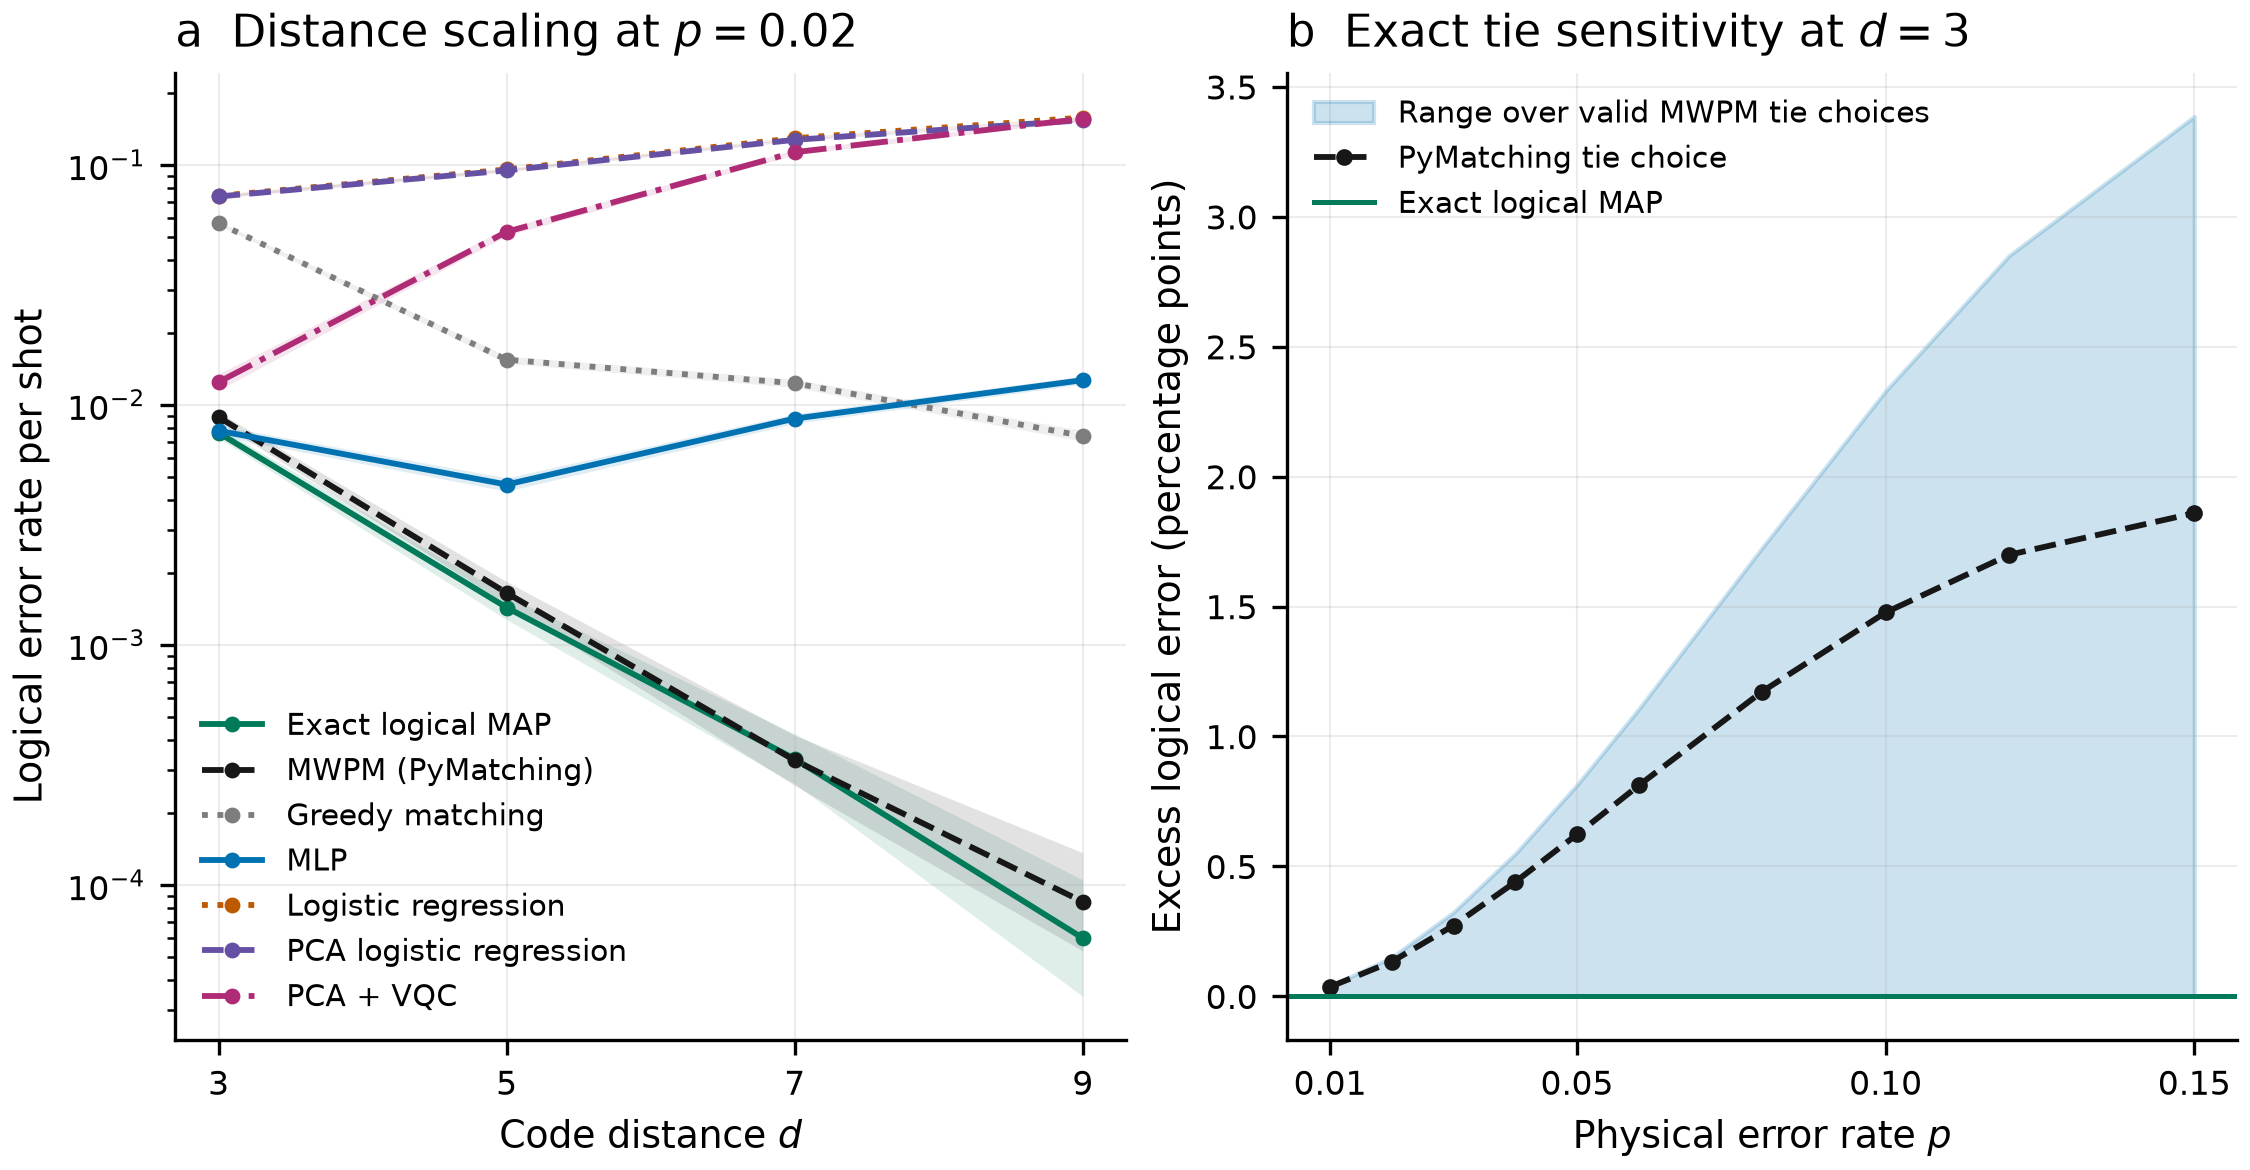
\includegraphics[width=\textwidth]{figures/ch6/qec_decoder_comparison_fig.png}
\caption[Distance dependence and matching ties]{Panel a shows the logical error rate against code distance at $p=0.02$ with Wilson $95\%$ intervals. Panel b shows the analytical excess error above exact MAP at $d=3$. The range spans the best and worst legal MWPM tie choices and the line shows the fixed PyMatching solution.}
\label{fig:ch6_comparison}
\end{figure}

The fraction of held-out shots whose detector string appeared in training
measures how often a test syndrome is familiar to a decoder trained on the
full $200{,}000$-shot pool. Table~\ref{tab:ch6_coverage} reports that fraction
at three physical error rates. At a fixed distance, the frequency of an exact
syndrome repeat depends strongly on noise. At $d=9$, $p=0.02$, the MLP errs
on $7$ of $84{,}932$ seen-pattern shots and $2{,}527$ of $115{,}068$
unseen-pattern shots. The conditional rates combine the effect of pattern
familiarity with differences in which patterns occur in each group.

\begin{table}[htbp]
\centering
\caption[Syndrome patterns shared by training and test shots]{Percentage of full test shots whose complete detector pattern appeared in the full training block. The artifact for this experiment also records counts and coverage at every sampled $p$.}
\label{tab:ch6_coverage}
\small
\begin{tabular}{rrrrr}
\toprule
\textbf{$d$} & \textbf{Detector bits}
& \textbf{$p=0.01$} & \textbf{$p=0.02$} & \textbf{$p=0.06$} \\
\midrule
3 & 8 & 99.989 & 99.992 & 99.990 \\
5 & 24 & 99.163 & 97.108 & 80.679 \\
7 & 48 & 94.202 & 77.621 & 11.637 \\
9 & 80 & 80.490 & 42.466 & 0.088 \\
\bottomrule
\end{tabular}
\end{table}

\section{The hybrid decoder}\label{sec:ch6_hybrid}

The VQC and PCA logistic regression use the same six principal components,
fit on the first $100{,}000$ training syndromes. The VQC uses means and standard
deviations from the first $15{,}000$ scores, clips standardised scores to
$[-3,3]$, and maps them to angles in $[-\pi,\pi]$. Logistic regression uses
unscaled scores and the full training block. The preprocessing uses only
training-block syndromes, including the VQC's validation inputs.
The comparison combines differences in predictor, input transforms and
training budget. An attribution to the circuit would require a nonlinear
classical control with the same preprocessing and training budget.
On the same $50{,}000$ test
shots at $d=3$, $p=0.02$, the VQC has $1.244\%$ logical error against $7.538\%$
for PCA logistic regression, $0.864\%$ for MWPM and $0.746\%$ for
exact MAP. At $d=9$ and the same $p$, the VQC and PCA logistic regression
have $15.554\%$ and $15.558\%$ error on the shared prefix. The fraction of
training variance retained by six components falls from $93.86\%$ at $d=3$
to $14.32\%$ at $d=9$ for this noise rate.

\section{Decoding cost}\label{sec:ch6_cost}

The timing column records batched CPU elapsed time per $1{,}000$ decoded
shots. It includes prediction-time preprocessing. The MWPM timer includes
graph construction, and the exact MAP timer starts after construction of
its likelihood tables. At $d=3$ it measures a lookup table over all
$256$ detector strings. The concurrent configurations, batch sizes
and initialisation conventions limit the timings to the implemented batch
workload. Single-shot latency under a syndrome-extraction cycle remains
unmeasured.

\section{Limitations and conclusion}\label{sec:ch6_limits}

The results cover phenomenological bit-flip faults on a repetition code. The
exact posterior supplies a reference for this known model at the tested
distances. Circuit-level noise, other error mechanisms, and codes with more
complex detector graphs require separate evaluation. The learned decoders are
trained per noise and distance configuration, and they receive flattened
detector strings or their PCA scores. These fits measure performance within
each configuration. Transfer across distances or noise rates remains outside
this evaluation. The VQC uses analytic state-vector readout, so its reported
LER applies to simulator inference.

The distance-3 enumeration permits a comparison with the full range of
minimum-weight tie choices. At larger distances, the posterior decoder
provides the same model-based accuracy reference without enumerating all
fault histories, although its state space still grows exponentially.

\end{document}
